%form: dc_form_03-04.tex ; user: dc_03-04_preparation_etc.tex
%========== DC =========
%===== p. 03-04 現在までの研究状況 =============
\section{現在までの研究状況}
\renewcommand{\refname}{}
%watermark: w03_past_dc
\newcommand{\研究の背景}{%
%begin  研究の背景===================
	\subsection{これからの研究計画の背景・問題点}
	\noindent
	●\textbf{これからの研究計画の背景・問題点}

	今後はこれまで開発したフェイクニュース早期発見モデルを発展させることで、
	拡散を抑制する。

	自然言語処理は、
	%前後の文脈を考慮できるBERT\cite{devlin-etal-2019-bert}や
	前節で述べたGrover\cite{NIPS2019_9106}を始め、
	より自然な文章が近年は生成できるようになった。
	前節の研究で実際にGroverを拡張し、\textbf{コメントを生成することで多くのフェイクニュースを早期検出}した。
	また、DNNは出力に対する説明を付加するモデルも開発されており\cite{shu2019defend}、
	早期検出との併用でユーザへの訴求力強化に繋がるものの、先行研究のいずれも行われていない。
	%しかしながら、速報性を併せ持つ説明可能な検出モデルは今の所先行研究のいずれも行われていない。

	%このことから今後は、\textbf{早期検出と説明の両面から拡散の抑制をより期待できるモデルの開発を目指す}。

	%\subsection{問題点}
	%\noindent
	%●\textbf{問題点}

	また提案モデルは多くのフェイクニュースの早期検出に成功したため、今後はFake誤判定を防止する。
	生成コメントを付加し分類した場合、提案モデルが検出したうち的中した割合である精度(Precision)は0.59だった(業績\red{3}-1)。
	%これは生成コメントを付加せず分類したときの0.68と比べ0.09ポイント下回った(業績\red{3}-1)。
	つまり\textbf{提案モデルがFakeと判断したユニット中、41\%はRealを誤って検出した}。
	精度と再現率の調和平均であるF値(F1 score)も提案モデルは目標値0.8に対して\textbf{0.68}であった。

	同時に、生成されたコメントは文法における不可解な点が多いため、生成コメントから判断の根拠とする説明可能性の提供は難しい。
	これではいくらフェイクニュースを検出できても、
	\textbf{判断の理由も説明できない狼少年めいたモデル}ではユーザの信用を得るのは難しく、拡散の抑制にはならない。

	\subsection{解決すべき点}
	\noindent
	●\textbf{解決すべき点}

	\textbf{分類性能向上}と、\textbf{不自然なコメントにより説明可能性を提供できない}2点を解決する必要がある。

	\subsection{着想に至った経緯}
	\noindent
	●\textbf{着想に至った経緯}

	本研究の目的である拡散の抑制を念頭に、
	実際に早期自動検出モデルをSNS上で運用する場合を想定し調査した。
	その結果、\textbf{フェイクニュース以上にユーザの信用を得なければ拡散を抑制できない}という課題を発見した。
	ゆえに\textbf{フェイクニュースを誤りなく多く早期検出する}よう性能を向上させることと、\textbf{説得力向上}のため説明可能性を提供すべきと着想に至った。

	{\footnotesize
		\begin{thebibliography}{99}
			\vspace*{-1mm}
			\setlength{\parskip}{0cm}
			\setlength{\itemsep}{0cm}
			\setcounter{enumiv}{6}
			\begin{spacing}{0.7}
				\bibitem{shu2019defend} Kai Shu, \textit{et al.} defend: Explainable fake news detection. In \textit{Proc. of the ACM SIGKDD}, 2019.
			\end{spacing}
			\end{thebibliography}
			
		%\bibliography{myreferences}
		%\bibliographystyle{junsrt}
	}
%end  研究の背景 ====================
}

\newcommand{\現在までの研究状況}{%
%begin  現在までの研究状況===================
	本研究では\textbf{フェイクニュースの早期自動検出}のために、\textbf{発信直後でコメントが少ないニュースを対象}に、真偽分類に取り組んだ。
	\textbf{真偽分類モデルにコメント⽣成モデルを導⼊}して、\textbf{コメントが少ない条件でもフェイクニュースの検出を可能に}した。

	\subsection{これまでの研究の背景}
	\noindent
	●\textbf{これまでの研究の背景}

	SNSの発展で、情報を迅速かつ大量に取得し、拡散することで容易に共有できるようになった。
	一方、悪意により他人を騙すために作られた\textbf{フェイクニュース}も拡散されやすくなった。
	ユーザの間で拡散されると、\textbf{騙された人々が社会的損害を起こす}ため、
	\textbf{\underline{フェイクニュース拡散の早期抑制が必要とされている}}。
	%例えば、2016年米国大統領選挙前にフェイクニュースに騙された人々がピザ屋で銃撃事件を起こした\cite{agencies_2016}。
	%特に今年はCOVID-19にまつわるフェイクニュースが広く拡散され、不安に陥った人々が買いだめを行うことが世界的に問題となった。
	%WHOは情報の過剰な氾濫を``インフォデミック''と定義し、テドロス事務局長は\textbf{誤った情報はウイルス以上に拡散されやすい}と指摘した\cite{ZAROCOSTAS2020676}。

	\subsection{問題点}
	\noindent
	●\textbf{問題点}

	現在フェイクニュースの拡散抑制のために、有識者が事実関係の確認を行う\textbf{ファクトチェック}がある。
	しかし属人的な作業で、拡散されてから着手されるため、結果を公表するまで時間がかかる。
	ゆえにあまり指摘が拡散されず、抑制に繋がらないことが多い。
	そこで自動で検出するために、ニュース内容や添付メディア、
	そしてユーザの反応からディープニューラルネットワーク (DNN)を利用する手法が提案されている
	\cite{Wang:2018:EEA:3219819.3219903}。
	特に、\textbf{ユーザの反応は真偽によって大きな違いがみられる}(i.e. フェイクである指摘やbotの介入)ため、\textbf{集合知として活用}した研究もみられる\cite{Wu:2018:TFF:3159652.3159677}。
	%これを自動で検出する場合、フェイクニュースは巧妙に実際のニュースを模した形をとるため、\textbf{単純なルールベース手法では難しい}。
	%近年ではニューステキストや添付メディア、ユーザの反応から\textbf{ディープニューラルネットワーク(DNN)}を利用した手法がみられる。
	%この場合はブラックボックス問題により\textbf{説明可能性が不足}するため、SNSユーザから支持を得にくい。
	%その中で\textbf{ユーザの反応は拡散後でしか得られない}ため、早期の検出を想定した場合はユーザの反応を評価対象にすることができない。
	しかし\textbf{ユーザの反応は拡散後でしか得られない}ため、\textbf{これらの⼿法ではフェイクニュースを早期検出できない}問題がある。

	\subsection{解決方策}
	\noindent
	●\textbf{解決方策}

	本研究は投稿コメント数が少なく、真偽の判別が難しい拡散初期段階のフェイクニュースの早期検出へ、
	%DNNの\textbf{学習時のみユーザの反応を活用}し、テスト時は
	\textbf{予想されるユーザの反応をコメント生成DNNモデルで生成・補完}
	し分類により実現した。

	\subsection{研究目的・研究方法}
	\noindent
	●\textbf{研究目的・研究方法}

	フェイクニュース早期検出へ\textbf{記事へのコメント生成で真偽分類性能が改善する}点を示す。
	本研究は本文1件と(モデル構造対応とデータ量確保の為)コメント3件を1ユニットとした。
	%コメント生成と真偽分類はそれぞれモデルを独立させた。
	図\ref{fig:model}の真偽分類でコメント1件欠損ユニットに、
	\textbf{生成による変化の比較}へ未補完時と\textbf{モデルが1件生成・補完}時を用意した。
	
	\begin{figure}[ht]
		\centering
		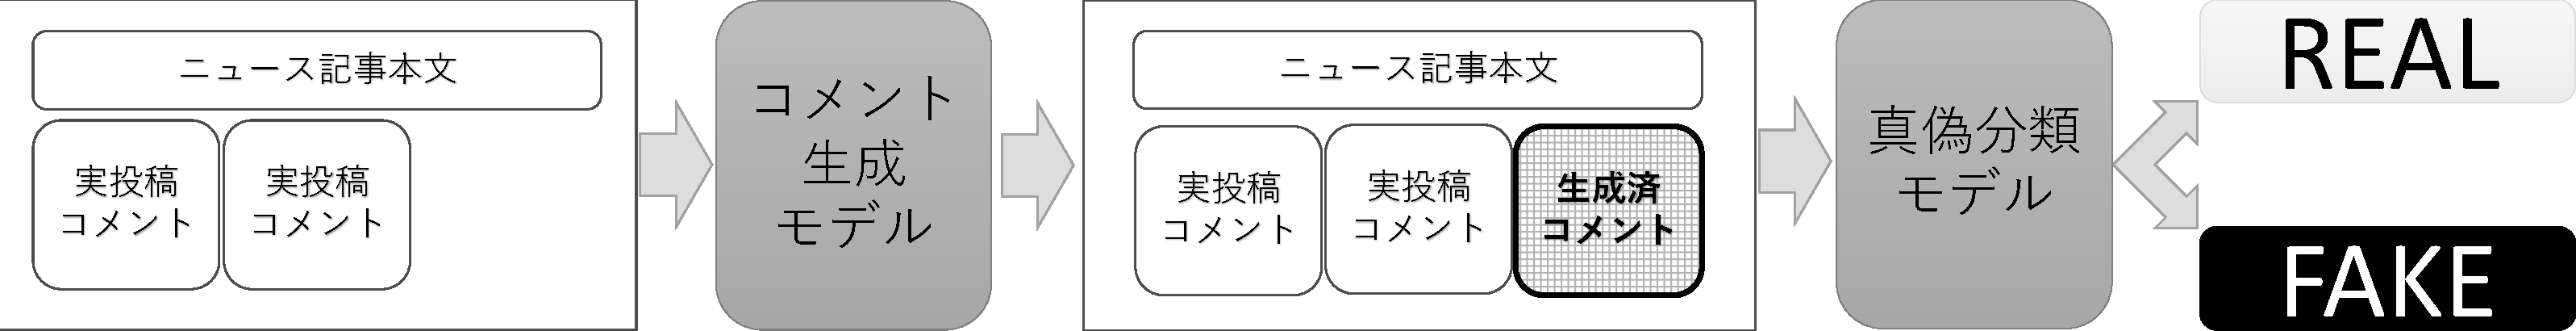
\includegraphics[width=0.95\linewidth]{figs/model.pdf}
		\vspace*{-3mm}
		\caption{提案手法の真偽判断までの流れ。}
		\label{fig:model}
	\end{figure}
	\vspace*{-4mm}
	\subsection{特色と独創的な点}
	\noindent
	●\textbf{特色と独創的な点}

	本研究の特⾊は、フェイクニュース拡散の傾向から記事に対するコメントの重要性に着目し、
	\textbf{早期発⾒のためにコメント⽣成モデルを導⼊}した点である。
	これで、生成コメントの調査で提案モデルが如何に真偽評価したか説明に足る情報が取得することで、
	ユーザに\textbf{真偽の判断理由の提供}も視野に入れられる。

	本研究の独創的な点は、\textbf{内容のみから予想されるコメントを生成する行為}が、
	%本研究では2点挙げられる。
	%1点目は申請者自らフェイクニュース拡散でみられる傾向から、
	%\textbf{ユーザの反応は確かに真偽を判断する有力な情報に足る上に、急速なSNS上の拡散への対応}を念頭に考案した点である。
	%2点目は\textbf{内容のみから予想されるコメントを生成する行為}そのものが、
	\textbf{真偽分類に有効な情報を提供するか解明}した点である。
	ゆえにこのこメント生成モデルは、真偽のみならずジョークニュースや認識不足に起因する誤報等も含めたマルチカテゴリ分類にも対応できる。
	%このため、\textbf{直接真偽を入力せずに記事とコメントから生成するよう独立モデル化}して、
	%真偽を評価する分類を補助させた。
	
	%\vspace*{-3mm}
	%\begin{itemize}
	%	\setlength{\parskip}{0cm}
	%	\setlength{\itemsep}{0cm}
	%	\item 自らフェイクニュース拡散の際に見られる傾向から手法の検討に入った点
	%	\item 拡散抑制の実現可能性を見据え、SNS上の拡散スピードに追いつくことがコンセプトである点
	%	\item \textbf{真偽を評価する分類タスクに、コメントの生成タスクを組み込んだ点}
	%	\item 分類性能を大きく失わずに速報性をもつことができる点
	%	\item 記事とコメントのみから真偽分類へ有用なコメントを生成するようモデル化した点
	%\end{itemize}
	%\vspace*{-2mm}

	%特に2点目が、先行研究ではみられない本研究最大の学術的特色であると申請者は考えている。

	\subsection{これまでの研究経過及び得られた結果}
	\noindent
	●\textbf{これまでの研究経過及び得られた結果}

	本研究はFakeNewsNet\cite{Shu2018FakeNewsNetAD, shu2017fake}を生成・分類用データセットとした。
	これはファクトチェックによって真偽評価済である英文ニュースと、それにTwitter上で言及された投稿(ツイート)等をもつ。
	本研究では3件以上英文ツイートが寄せられた芸能ニュースを真偽で各2000件使用した。
	拡散初期段階では多くのコメントを期待できないため、使用コメントは各3件ずつ無作為に選出し残りを対象から除外した。

	生成・分類モデルは、フェイクニュースを自動で作成するGroverモデル\cite{NIPS2019_9106}を拡張する形で実装した。
	このモデルはフェイクニュースをドメイン・著者・投稿日・見出し・本文の5要素に分け、いずれかの要素を\textbf{無作為に歯抜けにして予測させる形で生成学習を実現}したものである。
	今回はこれらの要素を\textbf{ユニットの4要素(記事本文と3件のコメント)に置換}し実装した。
	訓練が完了したコメント生成モデルを使い、図\ref{fig:model}の通り\textbf{コメントを1件欠損させたユニットに生成コメントを付加した上で、RealかFakeか分類させた}。
	分類モデルはGroverが提供した生成または実在を分類するモデルを教師あり真偽分類へ流用した。
	またコメント生成モデルが真偽そのものではなく、真偽に起因する文章の傾向差から学習させるため、
	真偽データはコメント生成モデルでは入力から除外し、分類モデルでのみ入力対象とした。

	その結果、提案モデルによって生成されたコメントを含めて分類した際、\textbf{Fake記事を見抜いた割合を示す再現率(Recall)が0.79}と、欠損のまま分類させたときの\textbf{0.75}を0.04ポイント上回った(業績\red{3?}-1)。
	これは本研究が目標としていた0.80に準ずる結果であった。
	今回は1件のみの⽣成であるため、再現率の上昇幅が限られていたが、⽣成するコメント数を増やすことで、
	⾼精度な判別の⽔準に達することが期待できる。
	%これは、\textbf{コメント生成によって疑わしい記事をより多く検出することを確認}した(業績\red{3?}-1)。
	%同時に、生成されたコメントで頻出した単語の傾向において真偽で大きな違いはみられなかった。
	%これは、\textbf{記事の真偽によってコメント内の単語傾向の差は軽微}であることを意味した。
	これは提案コメント生成モデルが、
	記事本文とコメントのみから信憑性による文章における傾向差異の学習に成功しており、
	\textbf{コメントが少ない段階でも真偽の判断が出来る可能性}を示唆した。
	この成果はフェイクニュースの早期発⾒に向けた足がかりとなる。

	なお業績\red{3?}-1において申請者は研究室から受けた技術的サポートを除き研究の全ての部分を担当した。
	%\vspace*{mm}

	{\footnotesize 
	%\bibliography{myreferences}
	%\bibliographystyle{junsrt}
	\begin{thebibliography}{99}
		%\vspace*{-2mm}
		\setlength{\parskip}{0cm}
		\setlength{\itemsep}{0cm}
		\begin{spacing}{0.6}
		%\bibitem{agencies_2016} Guardian staff and agencies. Washington gunman motivated by fake news `pizzagate' conspiracy,12 2016.
		\bibitem{ZAROCOSTAS2020676} John Zarocostas. How to fight an infodemic. \textit{The Lancet}, Vol. 395, No. 10225, p. 676, 2020.
		\bibitem{Wang:2018:EEA:3219819.3219903} Yaqing Wang, \textit{et al.} EANN: Event Adversarial Neural Networks for Multi-Modal Fake News Detection. In \textit{Proc. of KDD'18}, pp. 849-857. 2018.
		\bibitem{Wu:2018:TFF:3159652.3159677} Liang Wu and Huan Liu. Tracing Fake-News Footprints: Characterizing Social Media Messages by How They Propagate. In \textit{Proc. of WSDM '18},  pp. 637-645, 2018.
		\bibitem{Shu2018FakeNewsNetAD} Kai Shu, \textit{et al.} Fakenewsnet: Adata repository with news content, social context and dynamic information for studying fake news on social media. \textit{ArXiv}, Vol. abs/1809.01286, 2018.
		\bibitem{shu2017fake} Kai Shu, \textit{et al.} Fake News Detection on Social Media: A Data Mining Perspective. \textit{ACM SIGKDD Explorations Newsletter}, Vol. 19, No. 1, pp. 22-36, 2017.
		\bibitem{NIPS2019_9106} Rowan Zellers, \textit{et al.} Defending against neural fake news. \textit{NIPS 2019}, pp. 9054–9065, 2019.
		%\bibitem{EasyChair:3190} Yuta Yanagi, \textit{et al.} Fake news detection with generated comments for news articles. \textit{EasyChair Preprint no. 3190}, EasyChair, 2020.
		\end{spacing}
	\end{thebibliography}
	}
	%ぞうの卵はおいしいぞう。
ぞうの卵はおいしいぞう。
ぞうの卵はおいしいぞう。
ぞうの卵はおいしいぞう。
ぞうの卵はおいしいぞう。
ぞうの卵はおいしいぞう。
ぞうの卵はおいしいぞう。
ぞうの卵はおいしいぞう。
ぞうの卵はおいしいぞう。
ぞうの卵はおいしいぞう。
ぞうの卵はおいしいぞう。
ぞうの卵はおいしいぞう。
ぞうの卵はおいしいぞう。
ぞうの卵はおいしいぞう。
ぞうの卵はおいしいぞう。
ぞうの卵はおいしいぞう。
ぞうの卵はおいしいぞう。
ぞうの卵はおいしいぞう。
ぞうの卵はおいしいぞう。
ぞうの卵はおいしいぞう。
ぞうの卵はおいしいぞう。
ぞうの卵はおいしいぞう。
ぞうの卵はおいしいぞう。
ぞうの卵はおいしいぞう。
ぞうの卵はおいしいぞう。
ぞうの卵はおいしいぞう。
ぞうの卵はおいしいぞう。
ぞうの卵はおいしいぞう。
ぞうの卵はおいしいぞう。
ぞうの卵はおいしいぞう。
ぞうの卵はおいしいぞう。
ぞうの卵はおいしいぞう。
ぞうの卵はおいしいぞう。
ぞうの卵はおいしいぞう。
ぞうの卵はおいしいぞう。
ぞうの卵はおいしいぞう。
ぞうの卵はおいしいぞう。
ぞうの卵はおいしいぞう。
ぞうの卵はおいしいぞう。
ぞうの卵はおいしいぞう。
ぞうの卵はおいしいぞう。
ぞうの卵はおいしいぞう。
ぞうの卵はおいしいぞう。
ぞうの卵はおいしいぞう。
ぞうの卵はおいしいぞう。
ぞうの卵はおいしいぞう。
ぞうの卵はおいしいぞう。
ぞうの卵はおいしいぞう。
ぞうの卵はおいしいぞう。
ぞうの卵はおいしいぞう。
ぞうの卵はおいしいぞう。
ぞうの卵はおいしいぞう。
ぞうの卵はおいしいぞう。
ぞうの卵はおいしいぞう。
ぞうの卵はおいしいぞう。
ぞうの卵はおいしいぞう。
ぞうの卵はおいしいぞう。
ぞうの卵はおいしいぞう。
ぞうの卵はおいしいぞう。
ぞうの卵はおいしいぞう。
ぞうの卵はおいしいぞう。
ぞうの卵はおいしいぞう。
ぞうの卵はおいしいぞう。
ぞうの卵はおいしいぞう。
ぞうの卵はおいしいぞう。
ぞうの卵はおいしいぞう。
ぞうの卵はおいしいぞう。
ぞうの卵はおいしいぞう。
ぞうの卵はおいしいぞう。
ぞうの卵はおいしいぞう。
ぞうの卵はおいしいぞう。
ぞうの卵はおいしいぞう。
ぞうの卵はおいしいぞう。
ぞうの卵はおいしいぞう。
ぞうの卵はおいしいぞう。
ぞうの卵はおいしいぞう。
ぞうの卵はおいしいぞう。
ぞうの卵はおいしいぞう。
ぞうの卵はおいしいぞう。
ぞうの卵はおいしいぞう。
ぞうの卵はおいしいぞう。
ぞうの卵はおいしいぞう。
ぞうの卵はおいしいぞう。
ぞうの卵はおいしいぞう。
ぞうの卵はおいしいぞう。
ぞうの卵はおいしいぞう。
ぞうの卵はおいしいぞう。
ぞうの卵はおいしいぞう。
ぞうの卵はおいしいぞう。
ぞうの卵はおいしいぞう。
ぞうの卵はおいしいぞう。
ぞうの卵はおいしいぞう。
ぞうの卵はおいしいぞう。
ぞうの卵はおいしいぞう。
ぞうの卵はおいしいぞう。
ぞうの卵はおいしいぞう。
ぞうの卵はおいしいぞう。
ぞうの卵はおいしいぞう。
ぞうの卵はおいしいぞう。
ぞうの卵はおいしいぞう。
ぞうの卵はおいしいぞう。
ぞうの卵はおいしいぞう。
ぞうの卵はおいしいぞう。
ぞうの卵はおいしいぞう。
ぞうの卵はおいしいぞう。
ぞうの卵はおいしいぞう。
ぞうの卵はおいしいぞう。
ぞうの卵はおいしいぞう。
ぞうの卵はおいしいぞう。
ぞうの卵はおいしいぞう。
ぞうの卵はおいしいぞう。
ぞうの卵はおいしいぞう。
ぞうの卵はおいしいぞう。
ぞうの卵はおいしいぞう。
ぞうの卵はおいしいぞう。
ぞうの卵はおいしいぞう。
ぞうの卵はおいしいぞう。
ぞうの卵はおいしいぞう。
ぞうの卵はおいしいぞう。
ぞうの卵はおいしいぞう。
ぞうの卵はおいしいぞう。
ぞうの卵はおいしいぞう。
ぞうの卵はおいしいぞう。
ぞうの卵はおいしいぞう。
ぞうの卵はおいしいぞう。
ぞうの卵はおいしいぞう。
ぞうの卵はおいしいぞう。
ぞうの卵はおいしいぞう。
ぞうの卵はおいしいぞう。
ぞうの卵はおいしいぞう。
ぞうの卵はおいしいぞう。
ぞうの卵はおいしいぞう。
ぞうの卵はおいしいぞう。
ぞうの卵はおいしいぞう。
ぞうの卵はおいしいぞう。
ぞうの卵はおいしいぞう。
ぞうの卵はおいしいぞう。
ぞうの卵はおいしいぞう。
ぞうの卵はおいしいぞう。
ぞうの卵はおいしいぞう。
ぞうの卵はおいしいぞう。
ぞうの卵はおいしいぞう。
ぞうの卵はおいしいぞう。
ぞうの卵はおいしいぞう。
ぞうの卵はおいしいぞう。
ぞうの卵はおいしいぞう。
ぞうの卵はおいしいぞう。
ぞうの卵はおいしいぞう。
ぞうの卵はおいしいぞう。
ぞうの卵はおいしいぞう。
ぞうの卵はおいしいぞう。
ぞうの卵はおいしいぞう。
ぞうの卵はおいしいぞう。
ぞうの卵はおいしいぞう。
ぞうの卵はおいしいぞう。
ぞうの卵はおいしいぞう。
ぞうの卵はおいしいぞう。
  % << only for demonstration. Please delete it or comment it out.	
%end  現在までの研究状況 ====================
}

